\documentclass[a4paper,12pt]{article}
\usepackage[utf8]{inputenc}
\usepackage[croatian]{babel}
\usepackage{verbatim}
\usepackage{listings}
\usepackage{amssymb}
\usepackage{amsmath}
\usepackage{graphicx}
\usepackage{gensymb}
\usepackage{float}
\usepackage{algorithm}
\usepackage{algpseudocode}

\graphicspath{{../lab3/presentation/}}

\hyphenation{ray-marching}

\newcommand{\eng}[1]{(engl. \textsl{#1}\/)}

\author{Nikola~Bunjevac (0036485677)}
\title{Dokumentacija iz predmeta Računalna grafika\\{\normalsize 3. laboratorijska vježba}}

\begin{document}

\maketitle

\section{Raymarching}

Kao tema treće (samostalne) laboratorijske vježbe odabran je algoritam Raymarching. Glavna ideja
algoritma je iskorištavanje paralelizma grafičke kartice (GPU) kako bi se brzo moglo ``ispucati''
zraku za svaki piksel slike, odrediti njezino sjecište s površinom u sceni te primijeniti
osvjetljenje i prikazati rezultat. Možemo reći da je Raymarching algoritam srodan algoritmu
praćenja zrake \eng{raytracing}, ali za razliku od njega je aproksimativan. Provodi se unaprijed
određeni maksimalni broj iteracija i određuje se najmanja udaljenost duž ispucane zrake do neke površine.
Pseudokod je prikazan ispod.
\begin{algorithm}[H]
  \floatname{algorithm}{Algoritam}
  \caption{Funkcija Raymarch}
  \begin{algorithmic}[1]
    \Function{Raymarch}{vec3 $ro$, vec3 $rd$}
    \State float d = 0.0;
    \For{(int i = 0; i $<$ \texttt{MAX\_STEPS}; i++)}
    \State vec3 p = ro + d*rd;
    \State float dS = \Call{getDist}{p}; // funkcija udaljenosti
    \State d += dS;
    \If{(dS $<$ \texttt{SURFACE\_DIST} $||$ d $>$ \texttt{MAX\_DIST})}
    \State break;
    \EndIf
    \EndFor
    \State \Return d;
    \EndFunction
  \end{algorithmic}
  \label{alg:raymarch}
\end{algorithm}
Funkcija \verb|Raymarch| kao argumente prima točku u kojoj se nalazi kamera i vektor smjera
u kojemu će se zraka ispucati. U funkciji se izvodi petlja koja u najviše \verb|MAX_STEPS| koraka
određuje udaljenost najbliže površine (u smjeru zrake) od kamere. Važna komponenta je funkcija
\verb|getDist| pomoću koje modeliramo scenu. Ona vraća polumjer kružnice sa središtem u trenutnoj
točki duž zrake koja siječe najbližu površinu. To nam daje garanciju da se možemo pomaći duž zrake
barem za dužinu polumjera kružnice bez opasnosti da ``uđemo'' u neki objekt u sceni. Iterativnom
primjenom takvih pomaka, ili ćemo se približiti dovoljno blizu neke površine (\verb|SURFACE_DIST|)
i proglasiti sjecište, ili ćemo otići u beskonačnost.

Već smo spomenuli kako pomoću funkcije \verb|getDist| modeliramo scenu. Svi objekti u prostoru su
modelirani pomoću matematičkih funkcija što malo otežava modeliranje, ali nas ne ograničava u
kreativnosti. Tako primjerice možemo jednom funkcijom predstaviti kocku, drugom kuglu, trećom
torus itd. Također je funkcije moguće kombinirati raznim operacijama poput presjeka, unije,
deformacije i slično. Primjeri funkcija nalaze se na stranici\footnote{https://www.iquilezles.org/www/articles/distfunctions/distfunctions.htm}.

Korisno je napomenuti kako se sve iscrtava u stvarnom vremenu, uključujući i sjene. Njih dobivamo \textsl{gotovo
besplatno} tako da u točki sjecišta provjerimo je li izvor svjetlosti izravno vidljiv. Ukoliko
nije, taj piksel ćemo zatamniti kako bismo dobili dojam da se točka nalazi u sjeni.

\subsection{Struktura programa}
Program se sastoji od više funkcionalnih dijelova. Možemo ga podijeliti na glavni program koji
stvara prozor i uspostavlja OpenGL kontekst, prevodi i povezuje sjenčare te izvršava glavnu petlju
programa. Također je zadužen za slanje određenih informacija sjenčarima putem uniformnih varijabli.
Informacije koje se prenose su
\begin{itemize}
\item vrijeme proteklo od trenutka pokretanja,
\item položaj miša unutar prozora,
\item rezolucija prozora (visina i širina).
\end{itemize}

Možemo primijetiti kako je ova struktura slična usluzi Shadertoy\footnote{https://www.shadertoy.com/} što je bio i cilj glavnog programa--omogućiti jednostavnu lokalnu eksperimentaciju sa sjenčarima.
Kako bi se omogućilo iscrtavanje na cijelom prozoru, glavni program sjenčaru vrhova \eng{vertex shader} prosljeđuje
koordinate vrhova dvaju trokuta koji čine pravokutnik i zauzimaju cijelu površinu prozora.
Sjenčar vrhova jednostavno prosljeđuje podatke pa ni njega više nećemo razmatrati u nastavku.

Takva podjela omogućava nam da se usredotočimo na sjenčar fragmenata. Kako bismo mogli manipulirati pojedinim pikselima, možemo
koristiti dimenzije prozora i UV koordinate. Rezultat je brza povratna veza između promjene u
sjenčaru i rezultata na ekranu. Nema potrebe za ponovnim prevođenjem glavnog programa, a prevođenje
sjenčara traje vrlo kratko.

\subsection{Upute za pokretanje}

Program je pisan u programskom jeziku C++ i koristi OpenGL te biblioteku SDL2\footnote{https://www.libsdl.org/download-2.0.php}. Kao jedini argument prima putanju do sjenčara fragmenata kojeg izvodi.
Program pokrećemo naredbom
\begin{center}
\verb|./raymarching shader.frag|
\end{center}
nakon čega se otvara novi prozor i započinje iscrtavanje. Pomicanjem miša omogućeno je upravljanje
položajem izvora svjetlosti u sceni kako bi se pokazala interaktivnost, bez obzira što se većina
programa izvodi u sjenčaru na grafičkoj kartici.


\subsection{Primjeri}

\begin{figure}[h]
  \centering
  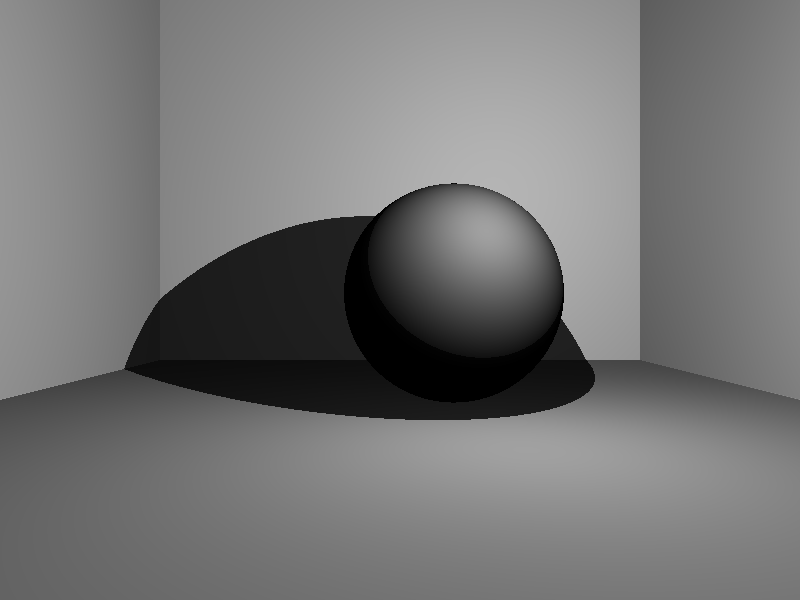
\includegraphics[width=\textwidth]{screen1.png}
  \caption{Jednostavna scena}
  \label{fig:simple}
\end{figure}

Slika \ref{fig:simple} prikazuje jednostavnu scenu u kojoj se nalazi kugla omeđena plohama.
Korištenjem miša možemo pomicati izvor svjetlosti i dobiti dozu interaktivnosti. Osim toga, kugla
se pomiče u sceni po unaprijed zadanoj putanji (pomoću matematičkih funkcija).

\begin{figure}[h]
  \centering
  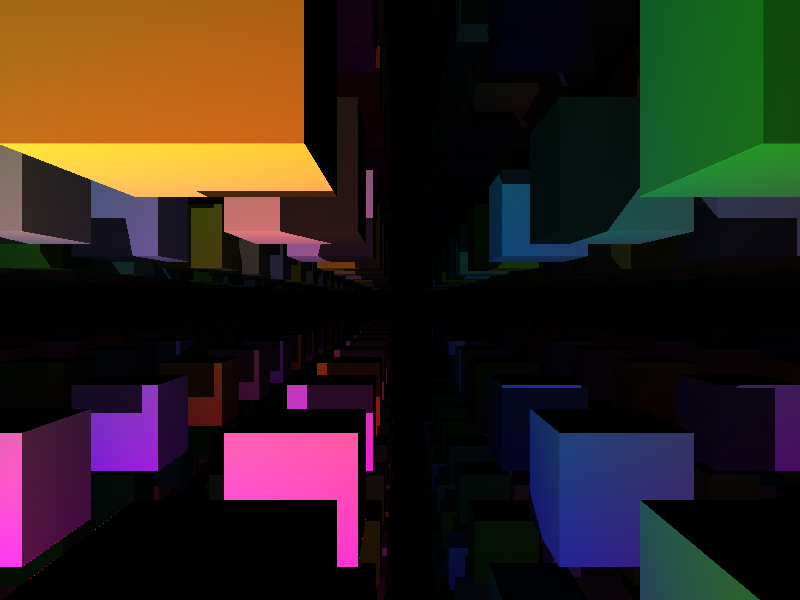
\includegraphics[width=\textwidth]{screen2.png}
  \caption{Puno objekata u boji}
  \label{fig:cubes}
\end{figure}

Na slici \ref{fig:cubes} možemo vidjeti ``beskonačno'' mnogo objekata/kocki u bojama. Kocke se
nalaze na cjelobrojnim koordinatama, a tako su i obojane--boja se primjenjuje ovisno o položaju u
prostoru. Slika \ref{fig:run} prikazuje primjer pokretanja gdje se u pozadini vidi kod sjenčara
fragmenata za pripadni primjer.

Također je moguće funkcijama modelirati i drugačije, složenije objekte. Primjer s torusima prikazan
je na slici \ref{fig:tori}, dok je apstraktniji primjer prikazan na slici \ref{fig:complex}.

\begin{figure}[h]
  \centering
  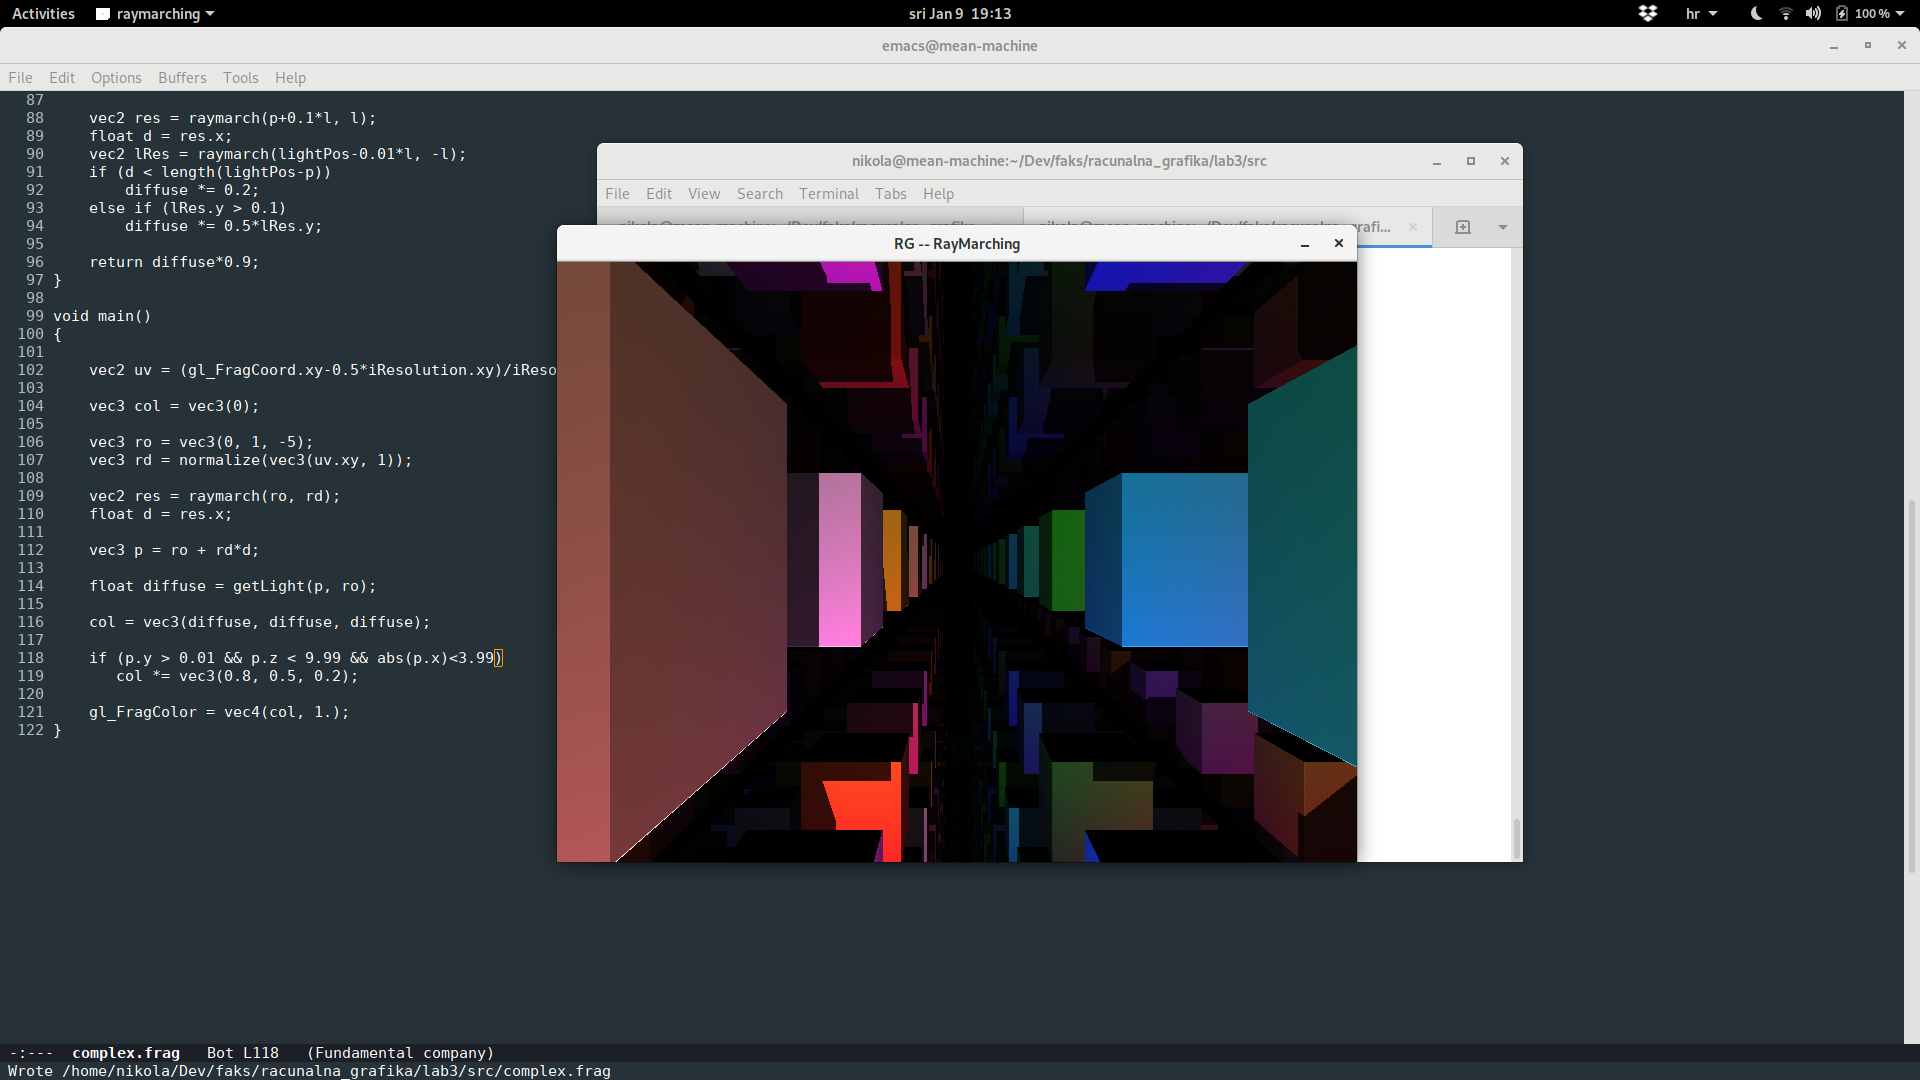
\includegraphics[width=\textwidth]{screen3.png}
  \caption{Primjer pokretanja programa}
  \label{fig:run}
\end{figure}

\begin{figure}[h]
  \centering
  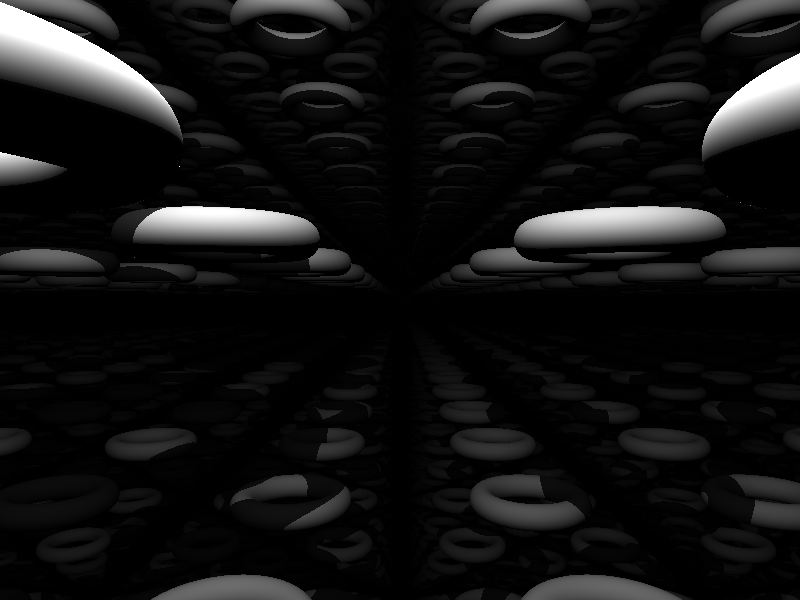
\includegraphics[width=\textwidth]{screen4.png}
  \caption{Primjer torusa}
  \label{fig:tori}
\end{figure}

\begin{figure}[h]
  \centering
  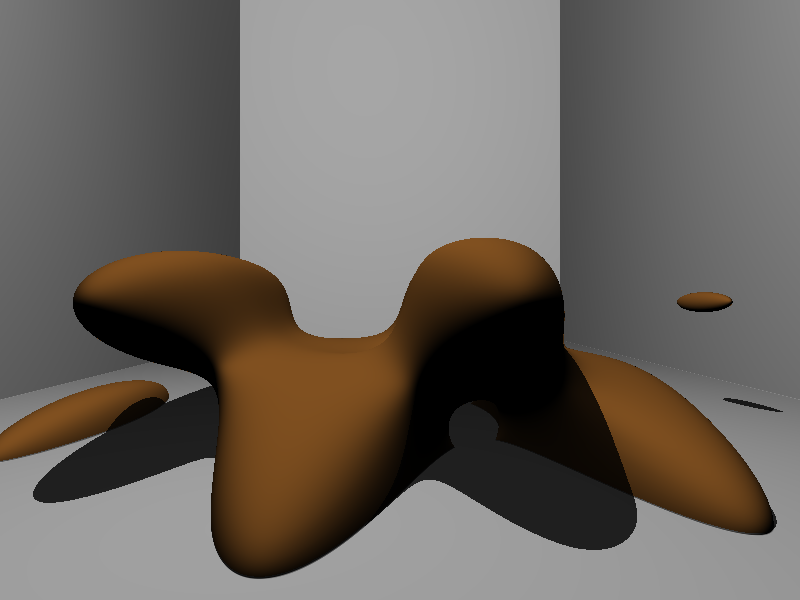
\includegraphics[width=\textwidth]{screen6.png}
  \caption{Scena s kompleksnim objektom}
  \label{fig:complex}
\end{figure}

\end{document}
